% ==================== Header ====================
\documentclass[12pt]{article} %montserrat fonts exists only in 10pt-12pt
\usepackage[a4paper, top=10mm, bottom=10mm, left=12mm, right=12mm]{geometry}
\usepackage[most]{tcolorbox}
\usepackage[hidelinks]{hyperref}
\usepackage[defaultfam,tabular,lining]{montserrat}
\usepackage{enumitem}
\usepackage{dirtytalk}
\usepackage{fontawesome5}
\usepackage{numprint}
\usepackage{setspace}

% ==================== Global settings ====================
\npdecimalsign{,} % Comma for decimals (European style)
\npthousandsep{.} % Dot for thousands (European style)
\setlength{\parindent}{0mm} % No paragraph indent
\pagenumbering{gobble} % No page numbering
\hyphenpenalty=100000 % No implicit hyphens
\exhyphenpenalty=100000 % No explicit hyphens
\tolerance=5000 % Avoid bad spacing
\emergencystretch=1em % Allow minor overshoots (trust me, looks better)

% ==================== Custom commands ====================
\definecolor{custom_blue}{RGB}{2,132,199}

\definecolor{linkedin_blue}{RGB}{10,102,194}

\newcommand{\NameText}[1] {{\Large\textbf{#1}}}

\newcommand{\HighlightedText}[1] {{\textbf{#1}}}

\newcommand{\PlaceAndTime}[2] {\HighlightedText{#1} \hfill \HighlightedText{#2}}

\newcommand{\SymbolAndLink}[3] {#1 \hspace{0mm} \href{#3} {\underline{#2}}}

\newcommand{\SymbolAndText}[2] {#1 \hspace{0mm} #2}

\newenvironment{ItemizeSection}[1]{
    \vspace{1mm}
    \HighlightedText{#1}
    \vspace{0.5mm}
    {\color{custom_blue} \hrule}
    \begin{itemize}[left=0.5em, topsep=0pt, itemsep=0pt, label={$\bullet$}]
}{
    \end{itemize}
}

\newenvironment{TextSection}[1]{
    \vspace{1mm}
    \HighlightedText{#1}
    \vspace{0.5mm}
    {\color{custom_blue} \hrule}
    \begin{itemize}[left=0.5em, topsep=0pt, itemsep=0pt, label={}]
}{
    \end{itemize}
}

\newenvironment{ItemizeSubsection}{
    \begin{itemize}[left=0.5em, topsep=-999pt, itemsep=0pt, label={$\circ$}]
}{
    \end{itemize}
}

% ==================== Name and Contact ====================

\begin{document}
\setstretch{1.5} % Spacing for the header
\begin{tcolorbox}[sharp corners=all, colback=custom_blue, coltext=white, frame empty, left=2mm, right=2mm, top=1mm, bottom=1mm]

    \noindent \begin{minipage}{0.6\textwidth}
        \NameText{Kyrylo Sovailo}

        \SymbolAndLink{\faAt}{k.sovailo@gmail.com}{mailto:k.sovailo@gmail.com} \\
        \SymbolAndLink{\faPhone*}{01763 5479038}{tel:+4917635479038} \\
        %\SymbolAndLink{\faGithub}{github.com}{https://github.com/kyrylo-sovailo} \\
        \SymbolAndLink{\faLinkedin}{linkedin.com}{https://linkedin.com/in/kyrylo-sovailo-19b4541b9} \\
        \SymbolAndText{\faEnvelope}{Pallaswiesenstr. 39, 64293 Darmstadt} \\
        %\SymbolAndText{\faAddressCard}{Staatsangehörigkeit: Ukraine} \\
        %\SymbolAndText{\faBabyCarriage}{Geboren am 08.10.2000 in Kiew, Ukraine} \\
        \SymbolAndText{\faBabyCarriage}{Geboren am 08.10.2000}

    \end{minipage}
    \begin{minipage}{0.39\textwidth}
        \raggedleft
        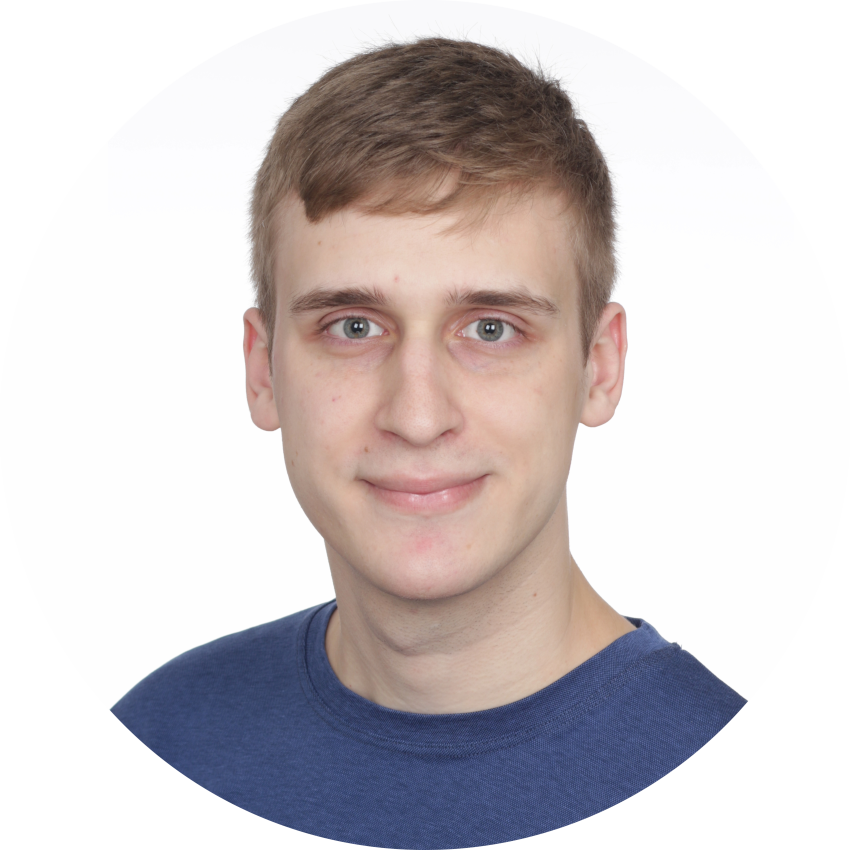
\includegraphics[width=50mm]{Photo_compressed_round.png}
    \end{minipage}
\end{tcolorbox}
\setstretch{1.1} % Spacing for the rest of the document

% ==================== Summary ====================

\vspace{-2.5mm}
\begin{TextSection}{Profil}
\item Zuverlässiger und sorgfältiger Mitarbeiter mit abgeschlossenem Masterstudium und Erfahrung in Softwareentwicklung sowie verwandten Bereichen. Ich arbeite gerne mit industriellen bzw. wissenschaftlichen Anlagen, bin aber bereit, neue Tätigkeiten zu erlernen.
\end{TextSection}

% ==================== Education ====================
\begin{ItemizeSection}{Ausbildung}
    \item \PlaceAndTime{Computational Engineering (CE) M.Sc.}{04.2023 -- 12.2025} \\
    \textbf{(Vertiefung Computational Robotics)} \\
    TU Darmstadt (Abschlussnote \numprint{2.1}) \\
    Abschlussarbeit (Note \numprint{1.7})

    \item \PlaceAndTime{Computational Engineering Science (CES) B.Sc.}{10.2018 -- 04.2023} \\
    RWTH Aachen University (Abschlussnote \numprint{2.4}) \\
    Abschlussarbeit (Note \numprint{1.7})

    \item \PlaceAndTime{Abitur}{09.2017 -- 09.2018} \\
     Studienkolleg an Freier Universität Berlin, technischer Kurs

    %\item \PlaceAndTime{Abitur}{09.2010 -- 05.2017} \\
    %Technisches Lyzeum der Nationalen Technischen Universität der Ukraine \say{Kiew Polytechnisches Institut}
\end{ItemizeSection}

% ==================== Professional background ====================
\begin{ItemizeSection}{Berufspraktische Erfahrungen}
    \item \PlaceAndTime{Studentische Hilfskraft an der Goethe Universität Frankfurt}{06.2023 -- 07.2024} \\
    Buchmann Institute for Molecular Life Sciences (BMLS)
    \begin{ItemizeSubsection}
        \item Softwarekonzipierung und -entwicklung, Anpassung der Software an die neue Hardware
        \item Umgang mit Laborgeräten
        \item Iterative Arbeit, Interpretierung von Benutzerfeedbacks
    \end{ItemizeSubsection}

    \item \PlaceAndTime{Praktikum bei Continental AG}{03.2022 -- 05.2022}
    \begin{ItemizeSubsection}
        \item Softwareentwicklung, Automatisierung von Arbeitsabläufen
        \item Mitarbeit in einem korporativen Umfeld
    \end{ItemizeSubsection}

    \item \PlaceAndTime{Studentische Hilfskraft an der RWTH Aachen University}{04.2021 -- 12.2021} \\
    Institut für Data Science im Maschinenbau (DSME)
    \begin{ItemizeSubsection}
        \item Inbetriebnahme und Test eines Roboterarms
        \item Entwicklung der Software für den Roboterarm
        \item Unterstützung der PhD-Studenten bei ihrer Forschung
    \end{ItemizeSubsection}
\end{ItemizeSection}

\newpage
% ==================== Skills ====================
\begin{ItemizeSection}{Fähigkeiten}
    \item Fortgeschrittener Umgang mit Computern
    \item Softwareentwicklung
    \item Grundkenntnisse in Hardwareentwicklung (CAD, PCB-Entwicklung)
    \item Erfahrung mit Robotern und Sicherheitsprotokollen
    \item Löten, Kenntnisse in Elektrik und Elektronik
    \item Umgang mit Geräten und Werkzeugen (Sägen, Bohrmaschinen, Kleinwerkzeugen)
\end{ItemizeSection}

\begin{ItemizeSection}{Persönliche Stärke}
    \item Zuverlässig und verantwortlich
    \item Sorgfältige und gewissenhafte Arbeitsweise
    \item Fähigkeit, selbstständig und in einem Team zu Arbeiten
    \item Hohe Lernbereitschaft
\end{ItemizeSection}

\begin{ItemizeSection}{Sprachen}
    \item Muttersprache: Ukrainisch
    \item Fließend (C1): Deutsch, Englisch
\end{ItemizeSection}

\begin{ItemizeSection}{Weitere Angaben}
    \item Führerschein: B1
\end{ItemizeSection}

\end{document}
